\chapter{Généricité et optimisation}\label{chap:chap1}

\epigraph{\foreignlanguage{USenglish}{How do we convince people that
    in programming simplicity and clarity --in short: what
    mathematicians call ``elegance''-- are not a dispensable luxury,
    but a crucial matter that decides between success and
    failure?}}{Edsger W. Dijkstra}
% Selected Writings on Computing: A Personal Perspective}, pp. 338-348


\clearpage

\section{Optimisation numérique et robotique}\label{sec:chap1_optim}

\subsection{Introduction à l'optimisation numérique}\label{sec:chap1_optim_intro}

\lettrine[lines=2, lraise=0.1, nindent=0em, slope=-.5em]%
{L}{a} robotique s'appuie sur différents outils mathématiques
pour résoudre les problèmes auxquels elle se trouve confrontée. Parmi
ces outils, l'optimisation numérique figure à une place de choix.


L'optimisation numérique est une branche des mathématiques permettant
de choisir automatiquement la meilleure solution parmi un ensemble de
solutions possibles. Les applications possibles couvrent des domaines
variés de la recherche opérationnelle aux statistiques et bien sûr la
robotique. Dans ce domaine particulier, l'optimisation numérique
permet par exemple d'optimiser un mouvement pour en améliorer
certaines caractéristiques ou bien encore trouver la prochaine
commande à envoyer aux moteurs du robot afin de réaliser une tâche
donnée.



Résoudre un problème d'optimisation numérique signifie trouver les
meilleurs paramètres résolvant le problème. Par meilleurs, il faut
entendre les paramètres minimisant la valeur d'une fonction de
coût. Intuitivement, on peut se représenter cette fonction comme un
indicateur de la ``qualité'' de la solution trouvée. Une solution
présentant un coût fort sera donc peu satisfaisante tandis qu'une
solution présentant un coût faible sera, elle, très attrayante. Tout
le raisonnement est ensuite fondé sur la linéarité -- au moins locale!
-- de cette fonction de coût. Plus simplement, près d'une mauvaise
solution, il n'y aura que des solutions légèrement meilleures et
légèrement pires, mais jamais trop différentes. De ce fait, il
``suffit'' de chercher dans quelle direction aller pour se diriger
vers les meilleures solutions pour finir par les trouver. Cette
approche implique une limitation majeure: si la fonction de coût n'est
pas convexe, on ne trouvera pas forcément la meilleure solution
globale -- parmi toutes les solutions -- mais ma meilleure solution
locale. C'est-à-dire qu'au voisinage de cette solution, toutes les
autres solutions sont de moins bonnes qualités. Dans cette situation,
tous les solveurs arrêtent leur recherche, mais rien ne garantit
qu'ailleurs il n'existe pas une autre solution de meilleure qualité.


Ce raisonnement permet de trouver les meilleurs paramètres pour un
problème donné, mais il est rare qu'une fonction de coût seule puisse
capturer complètement un problème donné. En fonctionnant de manière
indépendante du problème sous-jacent, on confère aux solveurs une
grande polyvalence. Mais par là même, il devient nécessaire
d'expliciter sous quelles conditions une solution au problème donné
est acceptable. Prenons un exemple: pour aller d'un point $A$ à un
point $B$ le plus rapidement possible, se déplacer avec une vitesse
infinie est sans aucun doute la solution optimale. Cependant, une
telle réponse ne présente guère d'intérêt dans la mesure où aucun
système physique ne sera en mesure de l'exécuter.


Deux stratégies peuvent alors être choisies. La première est
d'exprimer directement dans la fonction de coût cette information
supplémentaire. Dans le cadre de l'exemple précédemment cité, on
pourrait concevoir une fonction de coût réalisant la somme du temps de
déplacement et de la vitesse moyenne du robot. De ce fait, une vitesse
trop grande pénalise le résultat et par ce biais, le solveur tentera
plutôt de transformer la trajectoire géométrique plutôt que de jouer
sur la vitesse de déplacement du système. La limite de cette approche
est simple à comprendre: au fur et à mesure que les biais s'accumulent
-- le plus souvent en sommant les uns aux autres --, le coût initial
peut se retrouver ignoré par le solveur, car numériquement
négligeable. La fonction de coût n'a alors plus aucune justification
physique et ses variations peuvent devenir de plus en plus difficiles
à analyser pour le solveur.  Une seconde solution consiste à ajouter
des contraintes au problème. Ces contraintes sont exprimées sous la
forme d'équations ou d'inéquations déterminant si une solution donnée
est une solution acceptable. En robotique, des contraintes très
courantes sont les bornes sur les butées articulaires. Il est rare sur
un robot que les axes puissent se déplacer de manière totalement
libre. De ce fait, il est courant d'ajouter des contraintes inégalités
spécifiant que telle ou telle valeur de joint doit rester dans un
intervalle donné.


En exprimant comment résoudre un problème pratique via la construction
d'une fonction de coût $f$ et de contraintes $g_i > 0$,
\textbf{modélise} le problème afin qu'il soit soluble par optimisation
numérique. Ce procédé n'est pas trivial, car la qualité de la
modélisation impacte lourdement à la fois les temps de calcul et la
qualité du résultat final.



\subsection{Modélisation mathématique d'un problème}\label{sec:chap1_optim_model}


Résoudre un problème d'optimisation revient à trouver une solution pour:

\begin{equation}
  \min_{\mathbf{x} \in \mathbb{R}^n} f(x) \text{ sous la contrainte } \mathbf{x} \in \mathbf{X}
\end{equation}

où $f : \mathbb{R}^n \mapsto \mathbb{R}$ est la fonction de coût et
$\mathbf{X} \subset \mathbb{R}^n$ est l'espace des solutions
admissibles. Cet espace est habituellement défini par un ensemble de
contraintes égalités et inégalités:

\begin{equation}
  \mathbf{X} \equiv \left\{
  \begin{array}{l l}
    c_i (x) = 0    & \quad i \in \xi \\
    c_j (x) \leq 0 & \quad j \in \nu \\
  \end{array} \right.
\end{equation}

$c_i$, $c_j$ sont respectivement les ensembles de contraintes égalités
et inégalités. $i$ et $j$ des indices identifiant les contraintes.


L'optimisation numérique a pour objectif de développer des stratégies
-- algorithmes -- pouvant déterminer $\mathbf{x} \in \mathbf{X}$
minimisant les valeurs de la fonction $f$.


En absence d'arguments fort tel que la convexité de $f$ ainsi que des
contraintes $c_i, i \in \xi \cup \nu$, la solution $\mathbf{x}$
fournie par le solveur peut être un minimum local \index{minimum
  local}.


En effet, la plupart des méthodes d'optimisation tentent de trouver un
minimum en raffinant itérativement une solution à partir d'un candidat
initial $\mathbf{x_{\text{init}}} \in \mathbf{X}$. Le solveur, dès
lors, nécessite un critère d'arrêt à ce processus itératif. Ce critère
est donné par les conditions de Karush-Kuhn-Tucker \index{conditions
  de Karush-Kuhn-Tucker} ou conditions KKT.

\begin{mydef}\label{def:chap1_kkt}
Si $\mathbf{x} \in \mathbf{X}$ est un minimum local, alors il existe
$\lambda_i, i \in \xi$ et $\mu_j, j \in \nu$ des constantes non nulles
appelées multiplicateurs KKT tels que:
%
\begin{description}
\item[\textbf{Critère de stabilité}] \begin{equation}
  \nabla f(x) + \sum_{i \in \xi} \lambda_i c_i(x) + \sum_{j \in \nu} \mu_i c_i(x) = 0
\end{equation}
\item[\textbf{Critère de faisabilité primale}] \begin{equation}
\left\{
\begin{array}{l l}
  c_i (x) = 0    & \quad i \in \xi \\
  c_j (x) \leq 0 & \quad j \in \nu \\
\end{array} \right.
\end{equation}
\item[\textbf{Critère de faisabilité duale}] \begin{equation}
\mu_j \geq 0, j \in \nu
\end{equation}
\item[\textbf{Critère de complémentarité}] \begin{equation}
\mu_j c_j(x) = 0, j \in \nu
\end{equation}
\end{description}
\end{mydef}

Il est à noter que la Définition \ref{def:chap1_kkt} fournit des
conditions suffisantes afin de déterminer si un point est un minimum
local. Sous conditions de régularité, et dans le cas où le problème
est convexe, les conditions KKT sont nécessaires et suffisantes.


\subsection{Zoologie des solveurs}\label{sec:chap1_optim_solv}

\subsubsection{Zoologie mathématique}\label{sec:chap1_optim_solv_zoo}


Au-delà de cette présentation de la théorie générale, on peut
regrouper les techniques de résolution en différentes catégories
selon la difficulté des problèmes pouvant être traités. Nous ne nous
attarderons ici que sur les techniques d'optimisation
continues. Différentes caractéristiques peuvent rendre la résolution
plus délicate:
%
\begin{itemize}
\item Présence de contraintes,
\item Non convexité de la fonction de coût ou des contraintes,
\item Non linéarité de la fonction de coût ou des contraintes,
\item Fonction non -- ou mal -- définie en dehors des contraintes,
\item Variations numériques fortes entraînantes des erreurs numériques
  difficiles à juguler,
\item etc.
\end{itemize}
%
La combinaison de ces difficultés entraîne la classification des
solveurs dans de très nombreuses catégories dont un extrait est
détaillé dans le \autoref{tab:chap1_solver}.
%
\begin{table}
\begin{center}
\begin{tabular}{|>{\small}p{.24\textwidth}|>{\small}p{.305\textwidth}|>{\small}p{.305\textwidth}|}
\hline
\textit{Classe de problème} & \textit{Fonction de coût} & \textit{Contraintes}\\
\hline
\textbf{Moindres carrés linéaires} & $\sum_{i \in \{1, 2, \dotsc, n\}} (r_i - \mathbf{x}_i)^2$ où les $r_i$ sont des constantes & non \\
\hline
\textbf{LQP} \small{(opt. quadratique linéaire)} & quadratique & linéaire \\
\hline
\textbf{SQP} \small{(opt. non linéaire)} & non linéaire & non linéaire \\
\hline
\end{tabular}
\end{center}
\caption{Zoologie des problèmes en optimisation
  numérique. \label{tab:chap1_solver}}
\end{table}
%
Les algorithmes de résolution ont également des particularités
intrinsèques qui peuvent être particulièrement intéressantes dans le
cadre de la robotique. Par exemple, le démarrage à chaud ou ``warm
start'' \index{démarrage à chaud} \index{warm start|see{démarrage à
  chaud}} est la possibilité, pour un solveur, de résoudre
plusieurs problèmes à la suite tout en se souvenant de son état
interne afin de pouvoir gagner en temps de calcul lorsque le nouveau
problème est très proche du problème précédemment résolu. Cette
situation intervient notamment lorsque l'on optimise une trajectoire
tout en l'exécutant. L'optimisation se déroule pour différents
instants proches dans le temps pour lesquels l'évolution de l'état du
robot est minime. Une autre caractéristique est la capacité, pour un
solveur, de pouvoir être interrompu à n'importe quelle itération tout
en garantissant que la solution actuelle, bien qu'incomplète,
respecte la totalité des contraintes du problème. Ce comportement est
important lorsque l'optimisation est lancée dans un contexte où les
contraintes temporelles sont fortes, telles que dans le contrôleur
calculant les commandes du robot.



\subsubsection{Zoologie logicielle}\label{sec:chap1_optim_solv_zoosoft}


On l'aura compris: d'une théorie unique découle un ensemble
d'algorithmes pouvant résoudre des problèmes de complexité
variée. Plaçons-nous désormais à la place d'un roboticien devant
résoudre un problème particulier. Quels logiciels peut-il utiliser
pour se faire? Le Tableau \ref{tab:chap1_soft} détaille une partie
des paquets logiciels existants.
%
\begin{table}
\begin{center}
\begin{tabular}{|p{.24\textwidth}|p{.305\textwidth}|p{.305\textwidth}|}
\hline
\textit{Logiciel} & \textit{Classe de problème} & \textit{Caractéristiques}\\
\hline
\textbf{\href{http://devernay.free.fr/hacks/cminpack/index.html}{C/C++ MinPack}} & Moindres carrés linéaires & C/C++, réentrant, thread-safe \\
\hline
\textbf{\href{https://projects.coin-or.org/Ipopt}{Coin IPOPT}} & SQP & C++, réentrant \\
\hline
\textbf{\href{http://www.aemdesign.com/}{CFSQP}} & SQP & C, réentrant \\
\hline
\end{tabular}
\end{center}
\caption{Zoologie des problèmes en optimisation numérique. \label{tab:chap1_soft}}
\end{table}
%
Une conclusion s'impose au regard de cette liste de paquets logiciels:
les techniques les plus compliquées à implémenter sont peu disponibles
et il n'existe pas d'outil unifié permettant de résoudre différents
types de problèmes. Enfin, chaque outil traite une catégorie de
problème en particulier. Il est raisonnable de se demander si chaque
utilisateur lorsqu'il commence à définir son problème est à même de
choisir de manière pertinente le solveur -- et donc le framework --
adapté à son problème. Est-il certain que toutes les fonctions seront
différentiables et continues deux fois? Une fois? Est-on certain de ne
pas avoir besoin de contraintes inégalités, voire de ne pas avoir
besoin du tout de contraintes? Rien n'est moins sûr. Un exemple simple
est la gestion des collisions. On peut tout à fait développer un outil
robotique et le faire fonctionner dans un environnement ouvert avant
de vouloir s'attaquer à un problème plus difficile et prendre en
compte les collisions. Cela peut poser des problèmes extrêmement
importants, car le solveur ne sera pas le même dans les deux
cas. Cependant, il semble qu'avoir à réécrire, ou tout du moins
adapter, le problème précédent à une nouvelle bibliothèque logicielle
est inutile puisque finalement les deux problèmes se formalisent au
sein d'un même paradigme.


\section{De la dif\-ficulté à passer d'un paradigme uni\-que à une implémentation unifiée}
\label{sec:chap1_model2impl}


À première vue, il pourrait sembler que l'absence d'une architecture
unifiée pour la résolution de problèmes d'optimisation numérique est
le simple résultat d'un manque de volonté ou de coordination entre
concepteurs. Nous allons montrer ici qu'il n'en est rien. Une simple
agglomération des implémentations de différentes stratégies de
résolution ne saurait donner un ensemble cohérent et performant en
terme de temps de calcul sans une véritable réflexion sur comment
modéliser le paradigme décrit dans la \autoref{sec:chap1_optim}
tout en prenant en compte les limites internes des langages de
programmation. Nous allons tout particulièrement nous intéresser à la
programmation orientée objet qui est la fondation d'une large
proportion des langages modernes.


\subsection{Typage, programmation orientée objet et familles de types}
\label{sec:chap1_model2impl_typage}

\subsubsection{$\lambda$-calcul et théorie des types}
\label{sec:chap1_model2impl_typage_lambda}

Lors du développement de l'informatique, les langages de programmation
ont tout d'abord été de simples outils permettant de représenter du
code machine de manière succincte et plus facilement lisible par les
humains. Cependant, avec la complexification croissante des
applications, vérifier la correction des programmes est rapidement
devenu un enjeu critique. Pour se faire, les langages de programmation
ont progressivement adopté le typage comme moyen de n'autoriser que la
construction de programmes valides. Cette notion de type a issue de la
théorie des types \index{théorie des types}, une branche de la logique
mathématique. La première théorie unifiée des types a été développée
par Bertrand Russel \index{Bertrand Russel} au début du vingtième
siècle dans les \emph{Principia Mathematica} \citep{10.whitehead}.


Afin de démontrer les difficultés que peuvent poser la modélisation
d'un problème d'optimisation numérique, nous allons nous appuyer sur
un système de calcul formel particulier, le $\lambda$-calcul
\index{$\lambda$-calcul} inventé par Alonzo Church \index{Alonzo Church}
dans les années trente. Ce système de calcul formel a une expressivité
équivalente à une \index{Machine de Türing}. Nous allons tout d'abord
nous concentrer sur la construction des lambda-termes
\index{lambda-terme}, c'est-à-dire l'ensemble des expressions
syntaxiquement correctes pouvant être construites en lambda-calcul. Ces
lambda-termes peuvent être divisés en trois catégories: variables,
applications et abstractions. Les variables: $x$, $y$, \ldots Les
applications sont l'ensemble des expressions $u v$ où $u$ et $v$ sont
deux lambda-termes. Enfin les abstractions sont les expressions du
type: $\lambda x.u$ où $x$ est une variable et $u$ un
lambda-terme. Par exemple, l'application identité peut s'écrire en
lambda-calcul: $\lambda x.x$.


La procédure qui, à partir de n'importe quel lambda-terme, tente de la
simplifier en réalisant les applications par réécriture est appelée
$\beta$-conversion \index{$\beta$-conversion}. En réduisant un
lambda-terme, on réalise le calcul associé à ce dernier. Une propriété
utile serait de pouvoir déterminer si toutes les lambda-réductions
terminent, c'est-à-dire que l'on peut réduire tous les lambda-termes
jusqu'à un point où plus aucune réécriture \index{réécriture} n'est
possible.


Hélas, ce n'est pas le cas en lambda-calcul. Soit:

\begin{eqnarray}
  \Delta \equiv \lambda x.x\\
  \Omega \equiv \Delta \Delta \equiv (\lambda x.x) (\lambda x.x)
\end{eqnarray}

 On peut remarquer que la $\beta$-reduction de $\Omega$ boucle
 indéfiniment:

\begin{equation}
  (\lambda x.x) (\lambda x.x) =_{\beta} (\lambda x.x) (\lambda x.x)
\end{equation}

En terme calculatoire, on peut considérer que ce programme boucle et
ne termine jamais.


De ce constat, une autre interrogation se pose: peut-on construire un
sous-ensemble des lambda-termes normalisables? La réponse est oui, par
l'utilisation du lambda-calcul simplement typé \index{lambda-calcul
  simplement typé}. Dans cette version du lambda-calcul, toute
expression est annotée par un type. Les types sont de deux sortes:
$\iota$ et $\tau_1 \rightarrow \tau_2$ à condition que $\tau_1$ et
$\tau_2$ soient des types. $\iota$ représente le(s) type(s)
primitif(s) du langage permettant de représenter les booléens ou un
sous-ensemble des nombres entiers ou réels par exemple. Si $x$ est de
type $\iota$, on a alors:
%
\begin{equation}
  x \vdash \iota
\end{equation}
%
\ldots prononcé ``$\iota$ type $x$''. L'ensemble des types est quant à
lui noté $\Gamma$.


En définissant des règles de typage appropriées, on peut restreindre
les lambda-termes bien typés aux lambda-termes
normalisables. Cependant, une limitation de cette approche est qu'une
grande partie des expressions que l'on souhaiterait construire ne sont
pas correctement typées. En particulier, il n'est pas possible de
construire la fonction exponentielle dans ce paradigme.


\subsubsection{Programmation orientée objet et typage}
\label{sec:chap1_model2impl_typage_poo}

Indépendamment des systèmes de calculs formels, divers modèles plus
pratiques ont été développés au cours de la seconde moitié du
vingtième siècle. Notamment, la programmation orientée objet
\index{programmation orientée objet} a été introduite par Ole-Johan
Dahl \index{Ole-Johan Dahl} et Kristen Nygaard \index{Kristen Nygaard}
dans \index{Simula I} au cours des années soixante. Ce langage avait
pour but de permettre le développement de simulation à événements
discrets. Ce paradigme de pensée s'est progressivement développé
jusqu'à être massivement adopté par la majorité des langages de
programmation au cours des années quatre-vingt-dix. L'adoption massive
du C++ (Bjarne Stroustrup \index{Bjarne Stroustrup}, 1983) a participé
à la démocratisation de la POO.


La POO introduit la classe comme élément unitaire permettant la
conception d'un programme informatique. Alors qu'auparavant, une
séparation stricte était observée entre les données et les
algorithmes, une classe est un élément du langage regroupant ces deux
éléments. Les algorithmes fournis par une classe sont alors appelés
``méthodes'' tandis que les données prennent le nom
``d'attributs''. Cette réunification des données et des traitements
sur les données s'inscrit pleinement dans la lignée de la vision
informatique introduite par Von Neumann et l'architecture portant son
nom. L'innovation clé de cette architecture a été de permettre la
transmission sur un même bus des instructions composant un programme
ainsi que des données sur lesquelles les instructions vont
s'appliquer. On peut donc dire que la classe a poussé la réunification
algorithmes/données jusqu'à la conception interne des logiciels.

\begin{mydef}\label{def:chap1_type}
  Un type peut soit être un type fondamental noté $\iota$, soit un
  type fonctionnel, soit un type de classe. En pratique, il existe
  plusieurs types fondamentaux: réels, entiers, booléens, mais le
  nombre de types de base ne change en rien les règles de typage.
\end{mydef}

\begin{mydef}\label{def:chap1_class}
  Soit $\tau$ un type de classe. $\tau$ est défini par $a \in \mathfrak{A}_\tau$
  l'ensemble des attributs -- données -- de la classe et $m \in
  \mathfrak{M}_\tau$ l'ensemble des méthodes de la classe.

  \emph{Notation:} on notera $\tau.a$ l'attribut $a$ de la classe $\tau$ et
  $\tau.m$ la méthode $m$ de la classe $\tau$. Afin d'éviter les ambiguïtés,
  l'ensemble des symboles composant les éléments $\mathfrak{A}_\tau$ et
  $\mathfrak{M}_\tau$ sont disjoints.
\end{mydef}

\begin{mydef}\label{def:chap1_method}
  Soit $\mathfrak{M}_\tau$ l'ensemble des méthodes d'une classe. Une
  méthode $m$ du type de classe $\tau$ est une variable de type $\tau
  \rightarrow \tau'$ où $\tau'$ est un type quelconque.

  \emph{Notation:} L'application de la méthode $m$ de la classe $\tau$
  devrait s'écrire $a.m \tau$ où $a \vdash \tau$. Dans la mesure où
  l'on sait que $m \in \mathfrak{M}_\tau$, on peut se passer
  d'appliquer explicitement le premier argument du type fonctionnel et
  directement écrire $\tau.m$ pour signifier l'application de la
  méthode $m$.
\end{mydef}

\begin{mydef}\label{def:chap1_attribute}
  Soit $\mathfrak{A}_\tau$ l'ensemble des attributs d'une classe. Un
  attribut $a$ du type de classe $\tau$ est une variable de type
  $\tau'$ quelconque à l'exception des types fonctionnels prenant un
  type $\tau$ en argument.
\end{mydef}


\begin{myexample}\label{ex:chap1_class}
  Soit $A$ une classe définie par:

  \begin{equation}
    A \equiv \{ \underbrace{\{ \text{foo} \vdash \iota
      \}}_{\text{attribut}}, \underbrace{\{ \text{bar} \vdash A
      \Rightarrow \iota, \text{baz} \vdash A \rightarrow \iota
      \}}_{\text{méthodes}} \}
  \end{equation}

  $A$ possède un attribut et deux arguments. D'après la définition de
  $A$ et les
  Définitions \ref{def:chap1_method} et \ref{def:chap1_attribute}, on
  a:

  \begin{equation}
    a \vdash A \Rightarrow a.\text{foo} \vdash \iota
  \end{equation}

  \begin{equation}
    a \vdash A \Rightarrow a.\text{bar} \vdash A \rightarrow \iota
  \end{equation}
\end{myexample}


Cette représentation offre une vue d'ensemble intégrant à la fois des
données structurées et l'ensemble des opérations possibles sur ces
dernières. Auparavant, la séparation de ces deux éléments rendait plus
difficile la construction d'une vision globale: on ne pouvait, par
définition, pas connaître la liste des opérations définies sur un
groupe de données. Soit $\tau$ un type de classe, l'ensemble des
fonctions prenant $\tau$ en entrée n'est pas connu lors de la
compilation, car il peut être augmenté à tout moment d'un nouvel
élément en définissant une nouvelle routine. Il convient donc de
documenter la liste des opérations disponibles.

Inversement, il est souvent nécessaire d'augmenter le comportement
d'une classe en y ajoutant de nouvelles données et/ou de nouveaux
algorithmes. La POO modélise ce processus au travers de l'héritage de
classe. Soit $\tau_1$ un type de classe, $\tau_2$ un type de classe
héritant de $\tau_1$. On dit également que $\tau_2$ est un sous-type
de $\tau_1$, et est noté sous la forme:

\begin{equation}
  \tau_2 <: \tau_1
\end{equation}
%
%
Cette notion, proche de celle d'inclusion en théorie des ensembles,
permet de définir des familles de types interchangeables.
%
%
\begin{mydef}\label{chap1_oo_app}
  Soit $\Gamma$ un contexte de type. $\tau_1$, $\tau_2$, $\tau_3$
  trois types appartenant à ce contexte. La règle de typage des
  applications en programmation orientée objet est alors:


  \begin{equation}
    u v \text{bien formé} \Rightarrow u \vdash \tau_1 \rightarrow
    \tau_2 \wedge \tau_3 <: \tau_1
  \end{equation}

  Dès lors que $tau_3$ est un sous-type de $\tau_1$, les fonctions
  prenant en argument une variable de type $\tau_1$ acceptent
  également les arguments de type $\tau_3$.
\end{mydef}
%
\begin{mydef}\label{chap1_method_typing}
  Soit $\Gamma$ un contexte de type. $\tau_1$, $\tau_2$ deux types.

  On dit que $\tau_2 <: \tau_1$ si et seulement si:

  \begin{equation}
    \tau_2 <: \tau_1 \Leftrightarrow \mathfrak{A_{\tau_1}} \subset
    \mathfrak{A_{\tau_2}} \wedge \mathfrak{M_{\tau_1}} \subset
    \mathfrak{M_{\tau_2}}
  \end{equation}
\end{mydef}
%
Un sous-type se doit de contenir au moins tous les attributs et
méthodes de la classe dont elle hérite afin d'interdire la réécriture
vers des termes syntaxiquement faux. Le ``principe de substitution de
Liskov''\index{principe de substitution de
  Liskov} \citep{94liskov} définit, de manière équivalente,
la relation de sous-typage sous l'énoncé suivant:
%
\begin{mydef}\label{chap1_liskov}
  Si $q(x)$ est une propriété démontrable pour tout objet $x$ de type
  $T$, alors $q(y)$ est vraie pour tout objet $y$ de type $S$ tel que
  $S$ est un sous-type de $T$.
\end{mydef}


La Définition \ref{chap1_method_typing} introduit implicitement la
notion de polymorphisme d'héritage\index{polymorphisme!polymorphisme
  d'héritage}. Le polymorphisme\index{polymorphisme} est la capacité
pour un type fonctionnel de ne pas accepter en entrée un type unique,
mais une famille de types. Le polymorphisme le plus simple pouvant
être défini est la surcharge\index{surcharge}. Ce mécanisme autorise
la création de fonctions se réécrivant vers des $\lambda$-termes
différents selon le type de l'argument d'entrée. La formalisation de
ce système est décrite dans \citep{95castagna}.

Une autre forme de polymorphisme est le polymorphisme d'héritage. Si
$\tau_1$ et $\tau_2$ sont deux types tels que $\tau_2 <: \tau_1$ et
qu'il existe une méthode $m$ dans $\tau_1$ et $\tau_2$, alors tout
application de la méthode $m$ à un objet de type $\tau_2$ se réécrira
vers le $\lambda$-terme $\tau_2.m$. Un sous-type peut donc fournir une
réécriture alternative d'une fonction afin d'en spécialiser le
comportement.

La généralisation de cette propriété à toutes les fonctions au lieu
des méthodes uniquement permet d'obtenir le ``multiple
dispatch'' \citep{08muschevici}. Ce mécanisme est disponible dans un
nombre assez limité de langages de programmation, dont Common Lisp. En
effet, contrairement à la surcharge, le multiple dispatch ainsi que le
polymorphisme d'héritage nécessite une résolution à l'exécution qui
peut pénaliser l'implémentation des algorithmes. En limitant la
résolution dynamique au type du premier argument des méthodes, on
limite également le coût de la résolution à l'exécution. Ceci explique
en partie l'une des raisons pour lesquelles le premier argument des
méthodes est omis dans de nombreux langages de programmation. On
``masque'' par ce biais, le caractère spécifique de la résolution sur
le premier argument de la méthode et on peut, une fois ce premier
argument omis, considérer qu'il n'y a pas de résolution dynamique sur
les arguments des méthodes.


\subsubsection{Types paramétrés et génération de types}
\label{sec:chap1_model2impl_typage_param}

Face au coût induit par la résolution dynamique du polymorphisme par
héritage, on peut se demander s'il existe un moyen d'arriver au même
résultat sans ralentir l'exécution d'un algorithme. Une solution est
de générer des types afin de pouvoir déterminer à la compilation la
résolution des fonctions polymorphes. Ce mécanisme est appelé
``templates'' en C++ et se formalisent en $\lambda$-calcul sous la
forme de types paramétrés.


\begin{mydef}\label{chap1_parametrized_type}
  Un type paramétré est une fonction d'ordre supérieur $\text{type}
  \Rightarrow \text{type}$.

  \emph{Notation:} Soit $\tau$ un type paramétré. Le type $\tau$
  paramétré par $\alpha$ est dénoté $\tau_\alpha$. Il représente
  l'application du type $\alpha$ à la fonction d'ordre supérieure
  $\tau$.
\end{mydef}

Les types paramétrés permettent de définir un nouveau type de
polymorphisme, le polymorphisme
paramétré.\index{polymorphisme!polymorphisme paramétré} Ce
polymorphisme peut se formaliser en rendant les méthodes des classes
paramétrées dépendantes du paramètre de classe.

En pratique, ce type de polymorphisme est particulièrement
intéressant, car il n'induit pas de coût à l'exécution.


\subsection{Modélisation informatique du problème}
\label{sec:chap1_model2impl_typage_info}

La \autoref{sec:chap1_optim} a introduit le formalisme et les
outils que nous allons utiliser pour poser le problème de manière
formelle.


Un solveur est un algorithme qui prend en entrée un problème
d'optimisation et qui calcule un point dans l'espace des solutions.
Nous allons noter $\iota$ le type primitif représentant une partie des
réels et $[\iota]$ une liste de zéro, un ou plusieurs variables de
type $\iota$. $\tau_{\text{prob}}$ le type représentant le problème
d'optimisation. Nous allons voir comment ce type est habituellement
défini, introduire une paramétrisation alternative du problème fournie
par RobOptim et enfin montrer quelles avancées cette nouvelle
modélisation engendre.  Nous allons travailler en utilisant un solveur
générique qui sera dénoté:


\begin{equation}\label{eq:chap1_prob_type}
  \text{solv} \vdash \tau_{\text{prob}} \rightarrow \iota
\end{equation}


La vision habituellement implémentée consiste à définir un unique type
$\tau_{\text{prob}}$ dédié à un solveur précis. L'approche proposée
ici consiste, à la place, à définir une famille de types formée par
des classes, sous-classes éventuellement paramétrées pour tenter
d'exprimer la totalité de la théorie de l'optimisation numérique sous
la forme d'une et une seule modélisation.


\subsubsection{De la fonction\ldots au type fonctionnel?}
\label{sec:chap1_model2impl_typage_info_fct}


Naïvement, on pourrait penser qu'il n'y a rien de plus simple à
modéliser qu'une fonction mathématique. En effet, les types
fonctionnels ne sont-ils pas une transcription directe des fonctions
mathématiques habituelles? On aurait donc, à première vue:

\begin{equation}
  \begin{array}{ccccc}
    f & : & \tau_1 & \rightarrow & \tau_2\\
      &   & x      & \mapsto     & f(x)
  \end{array}
  \xhookrightarrow{\text{devient}}
  f \vdash \tau_1 \rightarrow \tau_2
\end{equation}

Cette modélisation convient, bien sûr, mais ne permet pas de ranger
les catégories en fonction selon leur nature: continue,
différentiable, etc.

En effet, pouvoir accéder au gradient de $f$ est primordial, mais
implémenter une fonction $\mathbf{\nabla}(f)$ est difficile car dans
de nombreux langages, dont celui utilisé par RobOptim -- C++ --, les
fonctions ne sont pas des objets de premier ordre et leur manipulation
est, de fait, mal-aisée.

Afin de pouvoir associer des métadonnées aux fonctions, une
représentation naturelle est l'utilisation d'une hiérarchie de classe.

Le critère choisi est la classe de la fonction: $\mathcal{C}^0$,
$\mathcal{C}^1$, \ldots à une nuance près. En effet, si une fonction
de classe $\mathcal{C}^n$ est déclarée, elle doit non seulement être
dérivable $n$ fois et continue $n+1$ fois, mais les valeurs des $n$
fonctions dérivées doivent pouvoir être calculées.

La classe de fonction associée à la possibilité de calculer les
gradients est un facteur très important lors de l'évaluation du
``niveau'' de difficulté d'un problème d'optimisation. Dès lors,
regrouper les fonctions selon ce critère semble être un choix
raisonnable.

\begin{mydef}\label{def:chap1_fcn}
  Soit $f$ une fonction mathématique continue dont on ne sait pas
  calculer la dérivée. Cette catégorie de fonctions est définie par la
  classe $\text{Fonction}$ définit par:

  \begin{equation}
    \text{Fonction} \equiv \{ \underbrace{\{ \#\text{entrée} \vdash
      \iota \}}_{\text{attributs}}, \underbrace{\{ \text{calcule}
      \vdash \text{Fonction} \rightarrow[\iota] \rightarrow \iota \}}_{\text{méthode}} \}
  \end{equation}

  L'attribut $\#\text{entrée}$ la cardinalité de l'espace d'entrée de
  la fonction et la méthode $\text{calcule}$ permets d'évaluer la
  fonction en un point. Nous ne traiterons ici que les fonctions dont
  l'espace de sortie est de cardinalité $1$. En effet, les fonctions
  dont l'espace de sortie sont de cardinalité $n$ peuvent être
  facilement représentables par $n$ fonctions dont l'espace de sortie
  est de taille $1$.
\end{mydef}

\begin{mydef}\label{def:chap1_derivfcn}
  Soit $f$ une fonction mathématique continue et dont on sait calculer
  la dérivée une fois. Cette catégorie de fonctions est définie par la
  classe $\text{FonctionDérivable}$ définit par:

  \begin{equation}
    \text{FonctionDérivable} \equiv \{ \{ \}, \{ \text{gradient}
    \vdash \text{FonctionDérivable} \rightarrow [\iota] \rightarrow [\iota] \} \} <: \text{Fonction}
  \end{equation}

  Le type $\text{FonctionDérivable}$ hérite du type $\text{Fonction}$
  et fournit, de surcroît, la méthode $\text{gradient}$ permettant
  d'évaluer le gradient de la fonction en un point.
\end{mydef}

\begin{mydef}\label{def:chap1_nderivfcn}
  Soit $f$ une fonction mathématique continue et dont on sait calculer
  la dérivée $n$ fois. Cette catégorie de fonctions est définie par la
  famille de classe $\text{Fonction}_n$ définit par:

  \begin{equation}
  \begin{split}
    \text{Fonction}_n \equiv
    \left\{
    \begin{array}{l l}
      \text{Fonction} & \quad \text{si $n = 0$}\\
      \text{FonctionDérivable} & \quad \text{si $n = 1$}\\
      \{ \{ \}, \{ \text{gradient} \vdash \text{Fonction}_n \rightarrow \iota \rightarrow [\iota] \rightarrow [\iota] \} \} <: \text{Fonction}_{n-1} & \quad \text{si $n > 1$}\\
    \end{array} \right.
  \end{split}
  \end{equation}

  On définit de sorte une famille de types formant une hiérarchie de
  classe sous la forme d'un peigne où $\mathcal{C}^n <:
  \mathcal{C}^{n-1} <: \dotsc <: \mathcal{C}^1 <: \mathcal{C}^0$.

  À partir de $\mathcal{C}^2$, on remarquera que la méthode
  $\text{gradient}$ est surchargée selon le nombre d'arguments. Avec un
  argument de type $[\iota]$, le gradient est évalué en un point. Avec
  deux arguments $o \vdash \iota$ et $\mathbf{x} \vdash [\iota]$, on
  aura pour $o \leq n$ le résultat de l'évaluation de la dérivée d'ordre
  $o$.
\end{mydef}


Cette hiérarchie de classe est le c\oe ur de la modélisation
informatique des problèmes d'optimisations, car elle permet d'exprimer
à la fois la fonction de coût et les contraintes éventuellement
présentes dans un problème. Il suffit alors à l'utilisateur souhaitant
définir sa fonction $F$ de le faire hériter du type adéquat de la
famille $\text{Fonction}_n$.

Cette approche sous forme de hiérarchie linéaire de classes en forme
de peignes a toutefois des inconvénients qui seront détaillés dans
la \autoref{sec:chap1_discussion} de ce chapitre.


\subsubsection{Des problèmes divers, un type unique}
\label{sec:chap1_model2impl_typage_info_prob}


Nous avons donc toute une famille de types définissant des fonctions
mathématiques: non seulement les $\text{Fonction}_n$ qui modélisent
les interfaces de notre programme, mais aussi tous les types
correspondant aux fonctions présentes dans un problème d'optimisation
particulier.

La question est désormais comment modéliser une ``classe'' de problème
d'optimisation numérique de manière générique tout en assurant une
sûreté maximum par typage.

La proposition réalisée ici est de définir une famille de types
$\tau_{\text{prob}}$ paramétré par $n > 0$ type(s). Le premier définit
le type de la fonction de coût tandis que tous les autres définissent
les types de fonctions des contraintes.


\begin{mydef}\label{def:chap1_prob}
  Soit $\tau_{\text{prob}(\tau_1, \tau_2, \tau_3, \dotsc)}$ tel que
  $\tau_i <: \text{Fonction}$, $i \in \{1, \dotsc, n\}$ par:

  \begin{equation}
  \begin{split}
    \tau_{\text{prob}(\tau_1, \tau_2, \tau_3, \dotsc)} \equiv
    \{ \{ & \text{coût} \vdash \tau_1,\\
    & \text{contraintes} \vdash [\cup_{i \in \{2, \dotsc, n\}} \tau_i],\\
    & \text{bornes\_contraintes\_min} \vdash [\iota], \\
    & \text{bornes\_contraintes\_max} \vdash [\iota] \},\\
    & \{ \} \}\\
  \end{split}
  \end{equation}

  Un problème d'optimisation est constitué d'une fonction de coût de
  type $\tau_1$ et un ensemble de fonctions pouvant être de type
  $\tau_i$, $i \in \{2, \dotsc, n\}$. Cet ensemble de fonctions
  associé à un ensemble d'intervalles permet de définir des
  contraintes égalité ou inégalité. Soit $\text{contraintes}_i$ la
  $i$-ème contrainte du problème, on a:

  \begin{equation}
    \text{bornes\_contraintes\_min}_i \leq \text{contraintes}_i \leq
    \text{bornes\_contraintes\_max}_i
  \end{equation}

  On notera que construire une contrainte égalité revient à spécifier
  une borne minimum et maximum identique.
\end{mydef}


La Définition \ref{def:chap1_prob} permet donc de modéliser un
problème d'optimisation numérique via l'utilisation d'un type
paramétré générique. Cette modélisation couvre une large partie des
problèmes d'optimisation avec ou sans contrainte tout en fournissant
une interface unique. Nous sommes donc dans un cas où l'utilisateur
peut définir son problème de manière naturelle, sans avoir à partir
d'un solveur qui impose son formalisme spécifique.


\subsubsection{Le chaînon manquant: le solveur}
\label{sec:chap1_model2impl_typage_info_solv}


Évidemment, il ne saurait être question de terminer cette section sans
revenir une dernière fois sur le c\oe ur et l'âme du système: le
solveur. Dans la section précédente, nous avons construit un type
paramétré qui satisfait les contraintes énoncées au début de cette
section, voire \autoref{eq:chap1_prob_type}.


En effet, on peut construire un type paramétré par le type de problème
permettant de modéliser un solveur.

\begin{mydef}\label{def:chap1_solver}
  Soit $\text{Solveur}_{\tau}$ une classe paramétrée par un type $\tau$
  tel que $\exists n, \exists \tau_1, \dotsc, \tau_n, \tau <:
  \text{Problème}_{\tau_1, \dotsc, \tau_n}$ et défini par:

  \begin{equation}
    \text{Solveur}_{\tau} \equiv \{ \{ \}, \{ \text{résous} \vdash
    \text{Solveur}_{\tau} \rightarrow \tau \rightarrow [\iota] \} \}
  \end{equation}
\end{mydef}

La Définition \ref{def:chap1_solver} fournit la dernière famille de
types indispensables à la modélisation d'un problème d'optimisation
numérique. Nous allons désormais nous attacher à montrer que diverses
classes de problèmes d'optimisation peuvent être exprimées via cette
modélisation unique.


\section{Exemples de formalisation de classes de problème}
\label{sec:chap1_model2impl_typage_ex}


Afin d'illustrer de démontrer que le formalisme décrit dans la section
précédente peut réellement permettre de décrire des problèmes
d'optimisation de manière efficace et générique, nous allons
construire les types représentant trois classes de problèmes en
utilisant les familles de types décrites dans la section
précédente. Les trois classes choisies sont:

\begin{itemize}
\item moindres carrés linéaires
\item optimisation non linéaire: fonction de coût non linéaire,
  contraintes linéaires ou non linéaires. Le gradient des fonctions
  doit pouvoir être évalué.
\item optimisation non linéaire: fonction de coût non linéaire,
  contraintes linéaires ou non linéaires. Le hessien\index{hessien}
  des fonctions doit pouvoir être évalué (dérivée d'ordre 2).
\end{itemize}


\subsection{Moindres carrés linéaires}
\label{sec:chap1_model2impl_typage_ex_moindre}

Les moindres carrés linéaires\index{moindres carrés linéaires}
utilisent une fonction de coût suivant une structure très
particulière. Proposer un type modélisant cette structure est
possible:

\begin{mydef}\label{ex:chap1_linearfct}
  Soit $\text{FonctionLinéaire}$ un type tel que:
  $$\text{FonctionLinéaire} <: \text{Fonction}_2$$
\end{mydef}

Nous avons ici choisi de faire dériver les fonctions
linéaires\index{fonction linéaire} du type $\text{Fonction}_2$. Cela
ne correspond pas à la réalité mathématique dans la mesure où une
fonction linéaire est infiniment dérivable, la dérivée étant nulle à
partir de la seconde dérivation. Il n'est pas possible d'exprimer cet
état de fait au regard de la modélisation adoptée ce qui représente
une limite du modèle de typage proposé. En pratique, les fonctions
plus de deux fois dérivables ne présentent pas d'intérêt particulier
et cette limite ne pose donc pas de problèmes en pratique.

\begin{mydef}\label{ex:chap1_leastsquarefct}
  Soit $\text{MoindreCarré}$ un type tel que
  $$\text{MoindreCarré} <: \text{FonctionLinéaire}$$

  Pour rappel, la fonction s'exprime mathématiquement sous la forme:

  \begin{equation}
    \sum_{i \in \{1, 2, \dotsc, n\}} (r_i - \mathbf{x}_i)^2
  \end{equation}
  \ldots où les $r_i$ sont des constantes.

  Cette fonction peut se modéliser par le type suivant:
  \begin{equation}
    \text{MoindreCarré} \equiv \{ \{ r \vdash [\iota] \}, \{ \} \} <: \text{FonctionLinéaire}
  \end{equation}
  où l'attribut $r$ représente les $r_i$ de l'équation précédente.
\end{mydef}


Une fois ces types définis, il ne reste plus qu'à instancier les types
paramétrés avec un ensemble de paramètres adéquats.

\begin{myexample}\label{ex:chap1_leastsquare}
  Paramétrisation proposée:
  \begin{description}
  \item[Fonction de coût] $\text{MoindreCarré}$
  \item[Contraintes] non
  \item[Problème] $\text{Problème}_{\text{prob}(\text{MoindreCarré})}$
  \end{description}
\end{myexample}


\subsection{Optimisation non linéaire (gradient uniquement)}
\label{sec:chap1_model2impl_typage_ex_optimgrad}

Nous allons traiter ici la classe de problèmes suivante: la fonction
de coût est non linéaire et les contraintes séparées en deux types
distincts: linéaires ou non linéaires.

\begin{myexample}\label{ex:chap1_cfsqp}
  Afin de pouvoir décrire cette classe de problème, la paramétrisation des types choisie est la suivante:
  \begin{description}
  \item[Fonction de coût] $\text{Fonction}_1$
  \item[Contraintes linéaires] $\text{FonctionLinéaire}$
  \item[Contraintes non linéaires] $\text{Fonction}_1$
  \item[Problème] $\text{Problème}_{\text{prob}(\text{Fonction}_1, \text{FonctionLinéaire}, \text{Fonction}_1)}$
  \end{description}
\end{myexample}

\subsection{Optimisation non linéaire (gradient et hessien)}
\label{sec:chap1_model2impl_typage_ex_optimhess}

Si l'on définit la même classe de problème, mais en ajoutant la
possibilité d'évaluer les hessiens des fonctions non linéaires, on
obtient la paramétrisation suivante.

\begin{myexample}\label{ex:chap1_ipopt}
  Paramétrisation proposée:
  \begin{description}
  \item[Fonction de coût] $\text{Fonction}_2$
  \item[Contraintes linéaires] $\text{FonctionLinéaire}$
  \item[Contraintes non linéaires] $\text{Fonction}_2$
  \item[Problème] $\text{Problème}_{\text{prob}(\text{Fonction}_2, \text{FonctionLinéaire}, \text{Fonction}_2)}$
  \end{description}
\end{myexample}

FIXME:  méthodes virtuelles, union de types, interfaces


\section{Discussion}
\label{sec:chap1_discussion}


Dans les sections précédentes, un formalisme permettant de représenter
de manière unifiée les problèmes d'optimisation numérique a été
présenté. On peut se demander quel apport l'utilisation d'un paradigme
unique peut apporter. Dans la plupart des cas, les utilisateurs de
solveurs numériques partent d'un outil existant et tentent de
modéliser le problème à résoudre de sorte qu'il puisse être soluble
par l'outil choisi. Cette approche est critiquable, car chaque problème
possède une difficulté intrinsèque et l'on devrait au contraire
pouvoir dans un premier temps modéliser son problème puis choisir le
solveur adéquat une fois la modélisation correctement effectuée. De
plus, le travail de recherche comporte, par nature, une grande part de
prototypage rapide où pouvoir tester de nouvelles approches rapidement
est important. Dans ce type de situation, utiliser le solveur le plus
avancé de l'État de l'Art n'est pas toujours nécessaire et l'on peut
éventuellement choisir à dessin un solveur ``trop'' puissant pour le
problème à résoudre et sous-optimal en terme de temps de
calcul. Inversement, il est courant qu'après avoir commencé un travail
de recherche, on se rende compte qu'un solveur équivalent plus rapide
ou présentant de meilleures caractéristiques existe. Dans ce cas, il
est plus simple de l'intégrer à un formalisme existant plutôt que de
devoir adapter son problème à un logiciel alors qu'algorithmiquement
parlant il n'existe pas de différence notable. Pour terminer, il est
arrivé que l'on commence tout d'abord par poser un problème robotique
pour s'apercevoir qu'il serait bien mieux traité à l'aider d'un
solveur dédié. Il est courant donc de devoir écrire un nouveau
solveur, ou modifier un solveur existant, afin de pouvoir rendre le
traitement du problème plus rapide. Dans ce cas également, un
formalisme unique présente de nombreux avantages, notamment en terme
de temps de conception.


Cette modélisation présente toutefois un certain nombre de limites qui
peuvent être divisées en deux: les limites intrinsèques de la
modélisation et celles qui ont été imposées par le langage de
programmation choisi pour l'implémentation des algorithmes, à savoir
le C++. Ces dernières seront abordées dans
la \autoref{sec:chap1_discussion}.Concernant les limites de la
modélisation, différents éléments sont difficiles à modéliser.


La première limite se présente quand les variables d'optimisations
appartiennent à des espaces possédant des structures différentes. Un
exemple commun en robotique est le mouvement 2d sur un plan en
translation et rotation. Trois variables caractérisent ce mouvement:
$x$, $y$ et $\theta$. Les deux premières décrivent un point dans
l'espace euclidien tandis que la dernière représente une rotation et
appartient donc au groupe spécial orthogonal\index{groupe spécial
  orthogonal $SO(n)$} en deux dimensions $SO(2)$. La représentation
des éléments de cet espace utilisant des réels est, par nature,
discontinue à $2\pi$. En choisissant un type unique pour représenter
les variables d'optimisation, nous perdons la possibilité de réaliser
un traitement spécifique selon l'espace mathématique auquel appartient
la variable d'optimisation. Malheureusement, définir plusieurs types
pour définir des éléments de différents groupes mathématiques est
difficile. En effet, l'ensemble des variables d'optimisations n'est
alors plus un tableau de réels, mais un tuple contenant des éléments
des types différents. Il faut encore alors trouver un moyen de définir
les opérations de groupe de manière efficace afin que le solveur
puisse utiliser les opérations adéquates pour opérer sur le groupe
tout en préservant ces caractéristiques. Ce problème est bien plus
visible lorsque l'on travailler sur des rotations en trois dimensions,
$SO(3)$, pour lequel de nombreuses représentations existent. Par
exemple si l'on considérer les quaternions, on souhaite en général
conserver un quaternion unitaire ce qui induit une contrainte
supplémentaire qu'il faut pouvoir insérer dans le problème. La
différenciation également suit des règles particulières qui
représentent une branche des mathématiques appelée géométrie
différentielle\index{géométrie différentielle}.

La seconde limite concerne la représentation des fonctions. En effet,
le parti a été de se limiter à la représentation des fonctions de
$[\iota] \rightarrow \iota$ soit pour les réels de $\mathbb{R}^n
\rightarrow \mathbb{R}$. Ce choix de conception a été pour garder la
taille des résultats calculés sous contrôle. En effet, pour une
fonction quelconque, la représentation des dérivées partielles se fait
sous la forme d'une matrice jacobienne\index{jacobienne}, puis d'un
tenseur d'ordre 3 pour les hessiens. Les tenseurs\index{tenseur} sont
rarement utilisés par les solveurs, car ces objets de très grande
taille sont lourds à manipuler. Qui plus est, il n'est pas toujours
nécessaire d'évaluer toutes les valeurs des matrices ou tenseurs
représentant les dérivées partielles d'une fonction et de ce fait,
découper une fonction à valeurs vectorielles en plusieurs fonctions
scalaires peut avoir du sens afin de limiter les calculs effectués.


La troisième limite est liée à la définition des types paramétrés. Il
n'existe pas, a priori, de hiérarchie de classe entre deux types
résultant d'un même type paramétré. Prenons par exemple le cas de
l'optimisation non linéaire avec ou sans hessien: on a donc deux
classes de problèmes reliés par une relation d'ordre qui semble
naturelle: si l'on a la possibilité de calculer les hessiens, on
devrait pouvoir le donner à la fois aux solveurs nécessitant les
hessiens, mais également à ceux qui ne les utilise pas. La classe où
l'évaluation des hessiens est possible est donc une classe plus
``facile'' que la classe où l'on n'a que des gradients. On peut,
évidemment, transformer un problème avec hessien en problème sans
hessien, mais ce n'est pas aussi simple que ce à quoi on pourrait
s'attendre: soit $\tau$ un type paramétré et $\tau_1$ $\tau_2$ tel que
$\tau_2 <: \tau_1$, on n'a pas $\tau_{\tau_2} <:
\tau_{\tau_1}$. Autrement dit, les fonctions dérivent les unes des
autres pour former une hiérarchie de classes interchangeables, mais
pas les problèmes! Pour changer de solveur, il faut donc changer
instancier un type de problème différent et ensuite le passer au
nouveau solveur. Cela représente généralement un travail court et
facile, mais qui peut désarçonner les utilisateurs peu adeptes des
langages de programmation utilisant des règles de typage complexe.


Face à la liste de ces critiques, on peut s'apercevoir qu'un élément
manquant, car dépassant le cadre de ce travail, est l'absence de
système de calcul formel sous-jacent. Développer un tel système tout
en préservant un typage fort est une tâche ardue; de ce fait, un
compromis entre ergonomie et effort de modélisation a été trouvé pour
permettre la réalisation de ce travail. Comme tout compromis, il
handicape parfois l'expression de certains problèmes dont on aurait
souhaité garder une formalisation plus proche de leurs natures
mathématiques véritables.


\section{RobOptim: une suite logicielle pour l'optimisation numérique en robotique}
\label{sec:chap1_roboptim}


Cette formalisation a été implémentée sous la forme d'une suite
logicielle pour l'optimisation numérique en robotique. Le langage
choisi pour l'implémentation est le C++. Ce langage a la particularité
d'être multiparadigme dont un très fort support à la fois de la
programmation orientée objet, mais également de la
métaprogrammation\index{métaprogrammation}, c'est-à-dire la génération
de familles de types via l'utilisation des ``templates''. Ce dernier
point a été abondamment utilisé pour permettre de fournir une
infrastructure de calcul sans impacter la performance des solveurs
sous-jacents. En effet, il n'y a pas de coût à l'exécution induit par
l'utilisation des templates\footnote{À l'exception de quelques
  phénomènes impactant à la marge certains mécanismes de résolution
  dynamique. On pensera par exemple aux transtypages dynamiques
  ralentis par la prolifération des types engendrés par les mécanismes
  de métaprogrammation.} contrairement à l'utilisation de certaines
techniques de programmation orientée objet comme les méthodes
virtuelles. En effet, comme expliqué dans la section précédente, les
méthodes virtuelles nécessitent une résolution et leur appel est donc
plus coûteux qu'une fonction simple \citep{96driesen}.


RobOptim\index{RobOptim} est une suite logicielle dont les composants
peuvent être divisés en trois groupes:
\begin{description}
\item[le noyau\index{noyau}] fournissant les interfaces et les types nécessaires à
  l'implémentation de la formalisation décrite précédemment,
\item[les solveurs] implémentant les algorithmes de résolution pour un ou plusieurs,
\item[les couches ``métier''\index{couche métier}] dédiées à la
  robotique et fournissant des fonctions régulièrement utilisées pour
  résoudre des problèmes d'optimisation. En particulier, le problème
  choisi pour montrer l'intérêt de cette approche concerne
  l'optimisation de trajectoire de marche pour un robot humanoïde ce
  qui a motivé le développement d'un ensemble d'outils pour
  l'optimisation de trajectoires.
\end{description}

\begin{figure}
  \begin{center}
    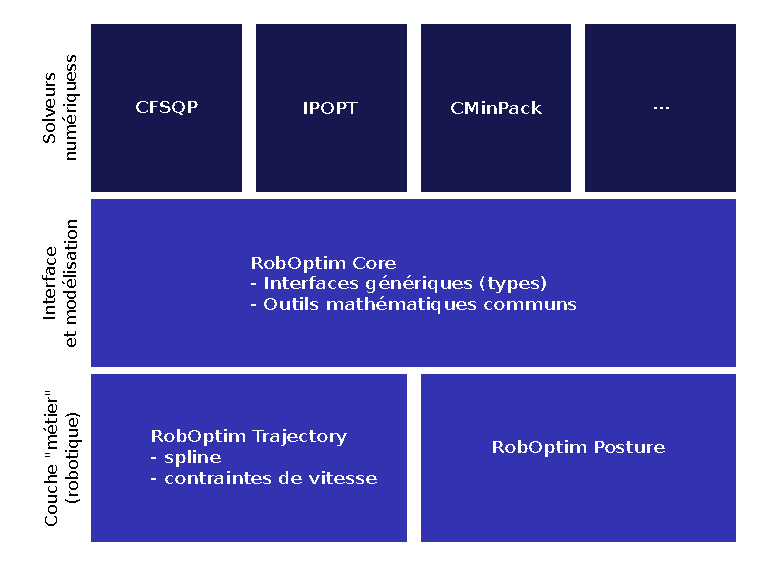
\includegraphics{src/chap1-roboptim/roboptim-architecture.pdf}
  \end{center}
  \caption{Architecture logicielle de RobOptim}
\end{figure}

\subsection{RobOptim core et ses plug-ins}
\label{sec:chap1_roboptim_plugin}

Le noyau de RobOptim fournit la modélisation mathématique des
fonctions, la classe définissant les problèmes d'optimisation ainsi
que les interfaces pour les solveurs. Le noyau, toutefois, ne contient
aucun algorithme de résolution. Ce paquet principal contient également
les outils mathématiques utiles pour résoudre les problèmes. Par
exemple, on peut augmenter le niveau de différenciabilité d'une
fonction via l'utilisation d'une méthode numérique se fondant sur la
méthode des différences finies. Cette méthode permet d'évalue la
dérivée d'une fonction en tirant des points aux alentours d'un point
de référence pour évaluer la courbure de la fonction aux alentours de
ce point. Plusieurs stratégies sont implémentées tirant deux ou cinq
points selon les cas. Cette fonctionnalité est implémentée via
l'utilisation du ``Design Pattern''\index{Design Pattern (motif de
  conception)} décorateur\index{Design Pattern (motif de
  conception)!Visiteur} tel que décrit dans le livre de
référence \citep{94gamma}. Ce motif de conception a la
particularité d'augmenter les capacités d'une classe sans en altérer
le comportement propre. Dans ce cas, cette classe paramétrée prend un
type de fonction en entrée, en hérite, tout en fournissant un niveau
de calcul supplémentaire des dérivées. D'autres outils permettent de
combiner des fonctions: les sommer, soustraire, multiplier entre elles
ou bien encore les combiner. Un autre décorateur fournit également un
cache afin d'éviter d'avoir à effectuer une nouvelle fois des calculs
lourds qui ont déjà été demandés précédemment.

Au-delà de la définition des fonctions, le noyau fournit l'interface
pour les solveurs. Deux solutions sont alors possibles: soit se lier à
une ou des bibliothèques tierces fournissant des algorithmes de
résolution, soit utiliser le système de plug-in\index{plug-in}
permettant d'en charger à l'exécution. L'objectif de ce système est de
pouvoir complètement déléguer au système la résolution d'un problème:
il y a un certain nombre de solveurs disponibles sur le système et
l'on pourrait ainsi, avoir une sélection automatique de l'algorithme
adéquat en fonction du type de problème en entrée. En pratique, ce
mécanisme autorise un changement de solveur pendant l'exécution du
programme.


\subsection{Les solveurs}
\label{sec:chap1_roboptim_solv}


Il est important d'insister sur le fait que ce travail n'a pas pour
but d'écrire un nouveau solveur ou bien de tenter d'apporter des
améliorations à une ou des approches existantes. La littérature du
domaine est foisonnante et bénéficie d'un effort de recherche
important. Toutefois, l'objectif final de ce travail reste la
possibilité d'utiliser dans un même paradigme plusieurs solveurs de
types différents. Des plug-ins RobOptim ont été écrits pour trois
solveurs:
%
\begin{description}
\item[CMinPack\index{CMinPack}] solveur permettant de résoudre des problèmes de type
  moindres carrés linéaires,
\item[CFSQP\index{CFSQP}] solveur pour les problèmes non linéaires, contraintes
  égalités et inégalités, calcul du gradient requis,
\item[IPOPT\index{IPOPT}] solveur pour les problèmes non linéaires, contraintes
  égalités et inégalités, calcul du gradient et hessien
  requis\footnote{Une version alternative qui ne nécessite pas le
    calcul du hessien est également fournie par le paquet logiciel.}.
\end{description}

Ces solveurs sont disponibles sous la forme de plug-in pour RobOptim
core et peuvent être chargés dynamiquement dans n'importe quel
problème d'optimisation RobOptim.


\subsection{Optimisation de trajectoires avec RobOptim}
\label{sec:chap1_roboptim_optim}

Un paradigme de programmation unifié permet également d'unifier les
outils de conception. En effet, l'écriture de bibliothèques de
fonctions de coût et de contraintes prend tout son sens une fois que
l'on a pu montrer que la même architecture est utilisable quelque soit
la structure du problème à résoudre. De ce constat, RobOptim s'est
enrichi d'une couche propre à la robotique, l'optimisation de
trajectoires.

Cette couche définit des trajectoires robotiques sous forme de
splines\index{spline}, c'est-à-dire de courbes
paramétrées\index{courbe paramétrée} par des points de
contrôle\index{point de contrôle}. Il est alors naturel de tenter de
vouloir altérer ces points de contrôle afin de raffiner le comportement
de la trajectoire: tenter de minimiser le temps nécessaire pour
réaliser le mouvement, ou l'énergie ou tout autre critère adéquat.

Cette bibliothèque fournit des bornes sur les vitesses du système à la
fois pour la vitesse de rotation et les vitesses linéaires. Le
problème d'optimisation de trajectoires est un problème semi-infini
dans la mesure où un souhait raisonnable est, par exemple, de borner
la vitesse du robot à tout moment de la trajectoire. Malheureusement,
la résolution de ce type de problèmes dans le cas général est
difficile et la technique la plus couramment utilisée reste une
discrétisation temporelle des contraintes. Ces stratégies présentent
l'inconvénient d'augmenter très largement le nombre de contraintes du
problème. De plus, le pas de discrétisation est difficile à évaluer et
a un très fort impact sur la vitesse de résolution. Enfin, si on
ajoute la possibilité d'accélérer ou de décélérer la trajectoire au
problème, le solveur peut tenter de changer la paramétrisation
temporelle afin de placer toutes les contraintes au début du mouvement
et pouvoir, par exemple, passer au travers d'un obstacle. Un tel
comportement peut être évité en attachant la contrainte non pas à un
moment temporel donné, mais plutôt à un point de la trajectoire
indépendamment de sa paramétrisation temporelle. Il suffit pour cela
de se donner une échelle fixe, de 0 à 1, représentant respectivement
le début et la fin de la trajectoire, et permettant aux contraintes de
se déplacer avec la reparamétrisation de la trajectoire. La
discrétisation de contraintes utilisant ce type de représentation est
supportée par RobOptim et permet de simplifier la résolution de
problèmes d'optimisation de trajectoires.


\section[Scénaro d'utilisation]{Scénaro d'utilisation: écriture d'une application robotique}
\label{sec:chap1_roboptim_scenario}


Afin d'illustrer les propos des sections précédentes, nous allons
désormais nous attacher à résoudre un problème de robotique avec le
paradigme de RobOptim. L'exemple choisi est un problème de robotique
humanoïde. Une stratégie possible pour pouvoir générer une trajectoire
de marche est de tout d'abord générer un ensemble d'empreintes de pas
et ensuite de générer un mouvement tel que le robot place
successivement ses pieds dans les empreintes de pas générées tout en
conservant son équilibre. Si cette stratégie est adoptée, le problème
initial se ramène à trouver une pile de pas appropriée pour passer
d'un point $A$ à un point $B$. Ce dernier problème se ramène lui-même
à trouver le mouvement sans collision dans le plan d'une boîte en
rotation et translation. Une fois cette trajectoire trouvée, il suffit
de placer les pas le long de la trajectoire de la boîte pour obtenir
la pile de pas souhaitée.


Pour planifier le mouvement de la boîte, nous avons choisi d'utiliser
un algorithme aléatoire de type RRT -- Rapidly exploring Random Tree
--. Cet arbre va tenter d'échantillonner l'espace $\mathbb{R}^2 \times
SO(1)$ des translations et rotation en deux dimensions tout en
validant que les configurations tirées ne violent pas de contrainte
ainsi que le chemin amenant du n\oe ud le plus proche au nouveau n\oe
ud tiré. Malheureusement, cette méthode rend des trajectoires rarement
réalistes et qui ne sont pas toujours acceptables. Il est donc courant
d'utiliser une méthode probabiliste pour trouver un premier chemin
évitant les collisions qui est ensuite amélioré dans une deuxième
passe réalisée par un algorithme d'optimisation. C'est cette seconde
passe que nous avons choisi d'exprimer dans le paradigme de RobOptim.


\subsection{Définition de la trajectoire et fonction de coût}
\label{sec:chap1_roboptim_cout}

\subsubsection{B-Splines et courbes paramétrées}
\label{sec:chap1_roboptim_cout_bspline}

Comme indiqué dans la section précédente, les trajectoires sont
définies sous la forme d'une courbe paramétrée. Ce type de courbe
appelé B-spline\index{spline!B-spline} est définie comme une
combinaison linéaire d'une famille de fonctions de base. Les deux
définitions ci-dessous permettent de calculer analytiquement ces
courbes et sont tirées de \citep{02malgouyres}.

\begin{mydef}\label{def:chap1_coxdeboor}
  Soit $n \in \mathbb{N}$, le nombre de points de contrôles. Soit $k
  \geq 1$, le degré des polynômes considérés. Soit $\Xi = (t_0, \dotsc,
  t_{n+k-1})$ un vecteur appelé, vecteur nodal avec $t_0 \geq \dotsc
  \geq t_{n+k-1}$. Les valeurs $t_i$ sont appelées noeuds. Les
  fonctions de base $N_{i,k}$ que nous allons définir, et donc les
  courbes B-splines que nous construirons ensuite, sont les
  polynomiales sur chaque intervalle $[t_i,t_{i+1}]$, pour $i =
  0,\dotsc,n-2$.

  La fonction $N_{i,k}$ est définie par récurrence\index{récurrence},
  comme suit:

  Pour $i = 0, \dotsc, n+k-2$, on pose:

  \begin{equation}
    N_{i,1}(t) = \left\{
  \begin{array}{l l}
    1 & \quad \text{si $t_i \leq t \leq t_{i+1}$ et $i = 0$ ou $t \neq t_i$} \\
    0 & \quad \text{sinon} \\
  \end{array} \right.
  \end{equation}

  Pour $r \geq 2$ et pour $i = 0, \dotsc, n + k - 1 - r$, on a la
  formule de récurrence:

  \begin{equation}
    N_{i,r}(t) = \frac{t - t_i}{t_{i+r-1}-t_i} N_{i,r-1}(t) +
    \frac{t_{i+r} - t}{t_{i+r} - t_{i+1}} N_{i+1,r-1}(t)
  \end{equation}

  La formule permettant de calculer les $N_{i,r}$ à partir des
  $N_{j,r-1}$ s'appelle la formule de Cox-de-Boor\index{Cox-de-Boor
    (formule de)}. Lorsque les dénominateurs de la formule s'annulent,
  on pose $\frac{0}{0} = 0$. C'est le cas lorsque plusieurs n\oe uds
  $t_i$ sont confondus.

\end{mydef}

\begin{mydef}\label{def:chap1_spline}
  Soit maintenant $P_0, \dotsc, P_{n-1}$ des points de contrôle. La
  courbe B-spline Q d'ordre $n$ et de degré $k - 1$ aillant $\Xi$ pour
  vecteur nodal et les $P_i$ pour points de contrôle s'exprime comme:

  \begin{equation}
    \left\{
    \begin{array}{ccc}
      Q : [t_{k-1},t_n] & \rightarrow & \mathbb{R}^3\\
      t & \mapsto & Q(t) = \sum_{i=0}^{n-1} P_i N_{i,k}(t)
    \end{array}
    \right.
  \end{equation}

  La courbe Q s'exprime donc comme une somme des fonctions $N_{i,k}$,
  pondérées par les points de contrôle.
\end{mydef}


Dans notre application, nous avons choisi d'utiliser des B-splines
uniformes de degré 3. Une B-spline est dit uniforme lorsque les
intervalles temporels entre les points de contrôle définis par le
vecteur nodal $\Xi$ est constant entre chaque point de contrôle. Dans
notre cas, cette valeur sera dénotée $\lambda$ et fera parti des
variables d'optimisation. Les autres variables d'optimisation sont les
points de contrôle eux-mêmes, soit trois variables par point de
contrôle: $(x,y) \in \mathbb{R}^2$ la position du robot dans le plan
et $\theta \in S^1$ l'orientation du robot. Le vecteur de variables
d'optimisation ainsi constitué est illustra par
la \autoref{tab:param}.

\begin{table}[htbp]
  \begin{center}
\begin{tabular}{|l|l l l|l|l l l|}
  \hline
  $\lambda$
  & $x_0$ & $y_0$ & $\theta_0$
  & \ldots
  & $x_n$ & $y_n$ & $\theta_n$ \\
  \hline
\end{tabular}
  \end{center}
  \caption{Variables d'optimisation du problème. \label{tab:param}}
\end{table}

\subsubsection{Fonction de coût}
\label{sec:chap1_roboptim_cout_cout}


La paramétrisation choisie permet d'accélérer la courbe. En effet,
plus la valeur de $\lambda$ décroît plus la courbe est
accélérée. L'objectif est alors simplement de tenter de réaliser le
mouvement le plus vite possible. On réalise alors une optimisation
temps minimal\index{temps minimal} utilisant la fonction de coût
suivante:

\begin{eqnarray}
\text{Coût}(\mathbf{x}) & = & (1, 0, \dotsc, 0)^T \mathbf{x}
\end{eqnarray}

Dans les faits, le solveur va progressivement saturer les contraintes
en accélérant la courbe. En particulier jusqu'à ce que la contrainte
de vitesse détaille ci-dessous, soit saturée. La \autoref{fig:speed}
montre le processus de saturation d'une contrainte sur la vitesse dans
le cadre d'une spline unidimensionnelle.

\begin{figure}[htbp]
  \begin{center}
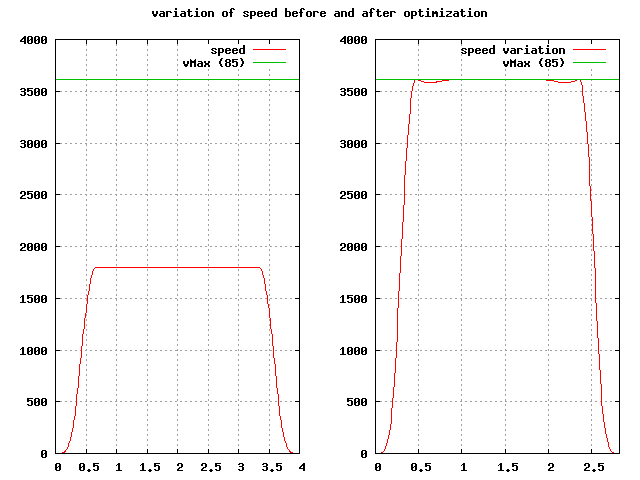
\includegraphics[width=\linewidth]{src/chap1-roboptim/time-optimization.png}
  \end{center}
  \caption{Saturation de la contrainte vitesse. \label{fig:speed}}
\end{figure}


\subsection{Contraintes}
\label{sec:chap1_roboptim_contraintes}

\subsubsection{Contrainte sur la vitesse}
\label{sec:chap1_roboptim_contraintes_vitesse}

\index{Contrainte!de vitesse} Le but de la contrainte sur les vitesses
est double: s'assurer de la correction de la trajectoire générée tout
en privilégiant la marche en avant par rapport à la marche sur le
côté. Outre l'aspect anthropomorphique, les robots humanoïdes ont un
comportement dégradé quand ils marchent ``en crabe''. L'espace
accessible par les jambes est réduit dans cette direction et la forme
des semelles du robot a tendance à le faire glisser dans ce cas. Les
contraintes sur les vitesses sont dupliquées afin de s'appliquer à la
fois au pied gauche et au pied droit. La formulation de la contrainte
pour tous les points de la trajectoire $t$ et pour chaque pied est:

\begin{equation}
  \begin{split}
  \forall t, \forall \text{pied} \in \{\text{gauche}, \text{droite}\}, &\\
  \text{ContrainteVitesse}_{(t,\text{pied})}(\mathbf{x}) & =
  (\frac{v_{\text{pied}}^{x}}{v_{\text{max}}^{x}})^2 +
  (\frac{v_{\text{pied}}^{y}}{v_{\text{max}}^{y}})^2 - 1
  \end{split}
\end{equation}

$v_{\text{pied}}^{x}$ et $v_{\text{pied}}^{y}$ étant respectivement
les vitesses frontales et orthogonales du pied
considéré. $v_{\text{max}}^x$ et $v_{\text{max}}^y$ respectivement les
vitesses frontales et orthogonales maximums du robot. Plus le ratio
$\frac{v_{\text{max}}^x}{v_{\text{max}}^y}$ est élevé, plus le robot
privilégiera la marche en avant pendant l'optimisation au détriment de
la vitesse d'exécution du mouvement.

Cette contrainte impose à la vitesse des pieds de rester dans une
ellipse allongée vers l'avant. Cette contrainte impose un mouvement
privilégiant la marche en avant et s'assure que le mouvement des pieds
est suffisamment lent pour pouvoir être jouée sur le robot. Afin
d'être certain que la contrainte est vérifiée en permanence, le temps
est discrétisé et on ajoute la contrainte pour tous les pas de temps.

\begin{figure}[htbp]
  \begin{center}
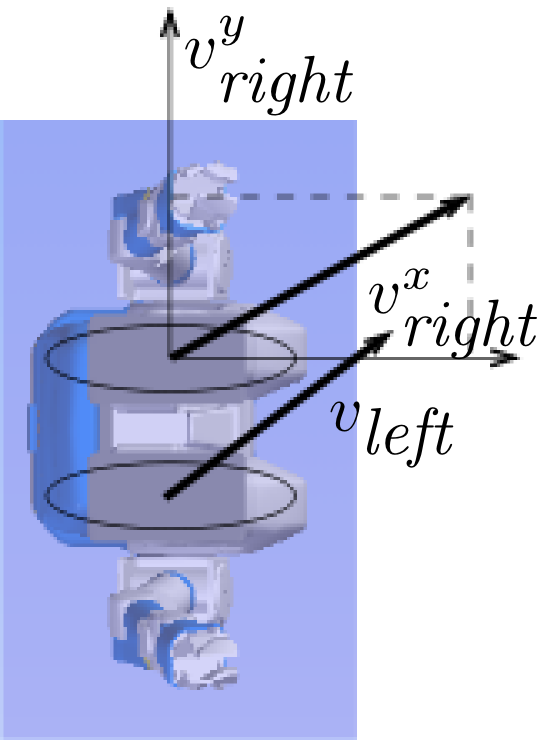
\includegraphics[width=5cm]{src/chap1-roboptim/speed-constraint-arrows.png}
  \end{center} \caption{Vitesses séparées du pied gauche et du pied
  droit. \label{fig:boxoptim}}
\end{figure}
\FloatBarrier


\subsubsection{Contrainte sur les obstacles}
\label{sec:chap1_roboptim_contraintes_obstacle}

\index{Contrainte!d'évitement des obstacles}
Les contraintes sur les obstacles se définissent naturellement: on
souhaite maintenir une distance minimale entre le robot et chaque
obstacle à tout moment. Comme avec la contrainte précédente, on
discrétise le temps afin de vérifier régulièrement la contrainte le
long de la trajectoire. La contrainte en tous points de la trajectoire
$t$ et pour tous les obstacles est la suivante:

\begin{eqnarray}
\forall t, \forall j, \text{Distance}(\mathcal{R}(t), \mathcal{O}_j) \geq d_{\min}
\end{eqnarray}

$\mathcal{R}$ représente ici la position du robot et $\mathcal{O}_j$
la position de l'obstacle $j$ de l'environnement. $d_{min}$ représente
une distance de sécurité déterminée empiriquement entre les obstacles
et le robot.


\subsection{Résolution et résultats expérimentaux}
\label{sec:chap1_roboptim_resultats}


La fonction de coût est une fonction linéaire, mais les contraintes
sont non linéaires. Il est nécessaire de définir des types RobOptim
pour ces fonctions, le type de problème associé:
$\text{Problème}_{\text{FonctionLinéaire}, \text{Fonction}_1}$. Le
gradient analytique a été déterminé pour toutes les fonctions afin
d'accélérer les calculs. La \autoref{fig:obstacle} montre
un exemple de chemin optimisé par le solveur CFSQP en simulation et
la \autoref{fig:results} un exemple d'application sur le
robot. Le \autoref{tab:benchmarks} illustre les temps de calcul
rencontrés sur deux scénarios.

% Les calculs des fonctions et des gradients associés sont détaillés dans FIXME

\begin{figure}[htbp]
  \begin{center}
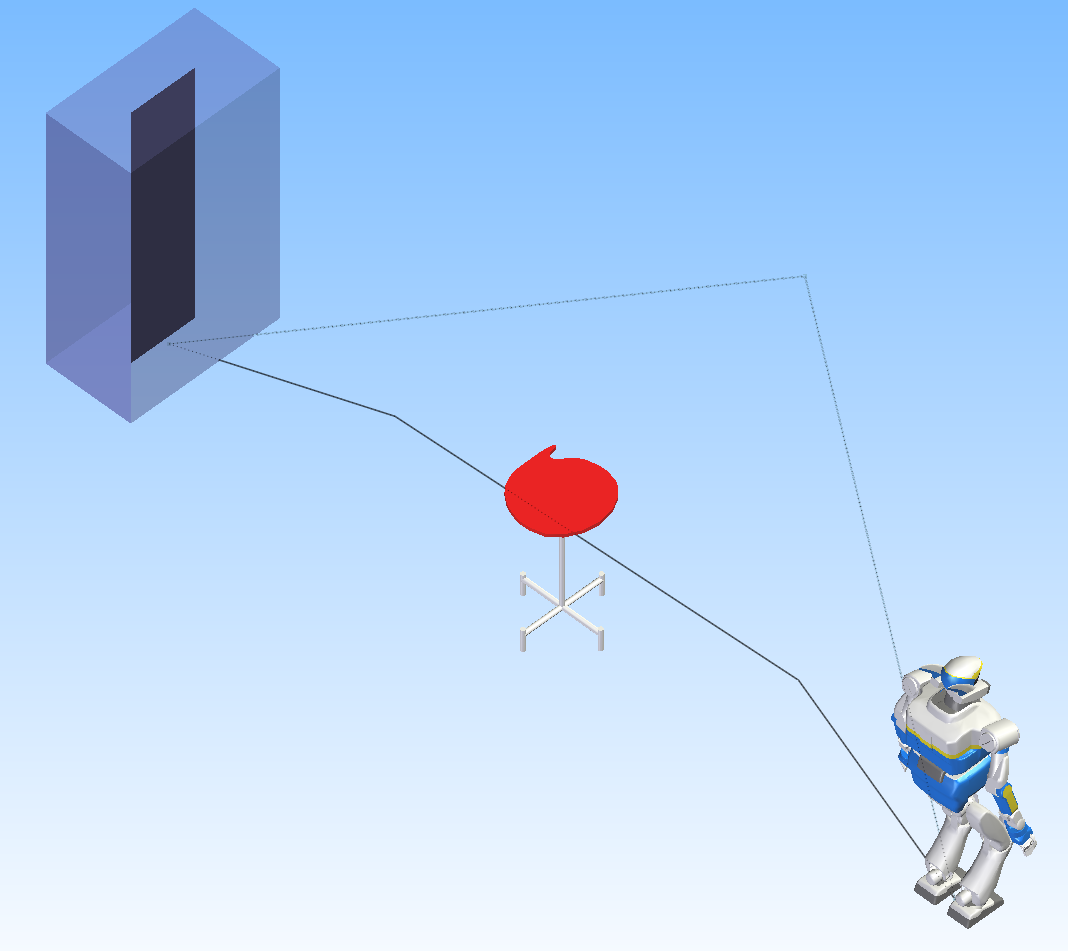
\includegraphics[width=.8\linewidth]{src/chap1-roboptim/straight-line-obstacle.png}
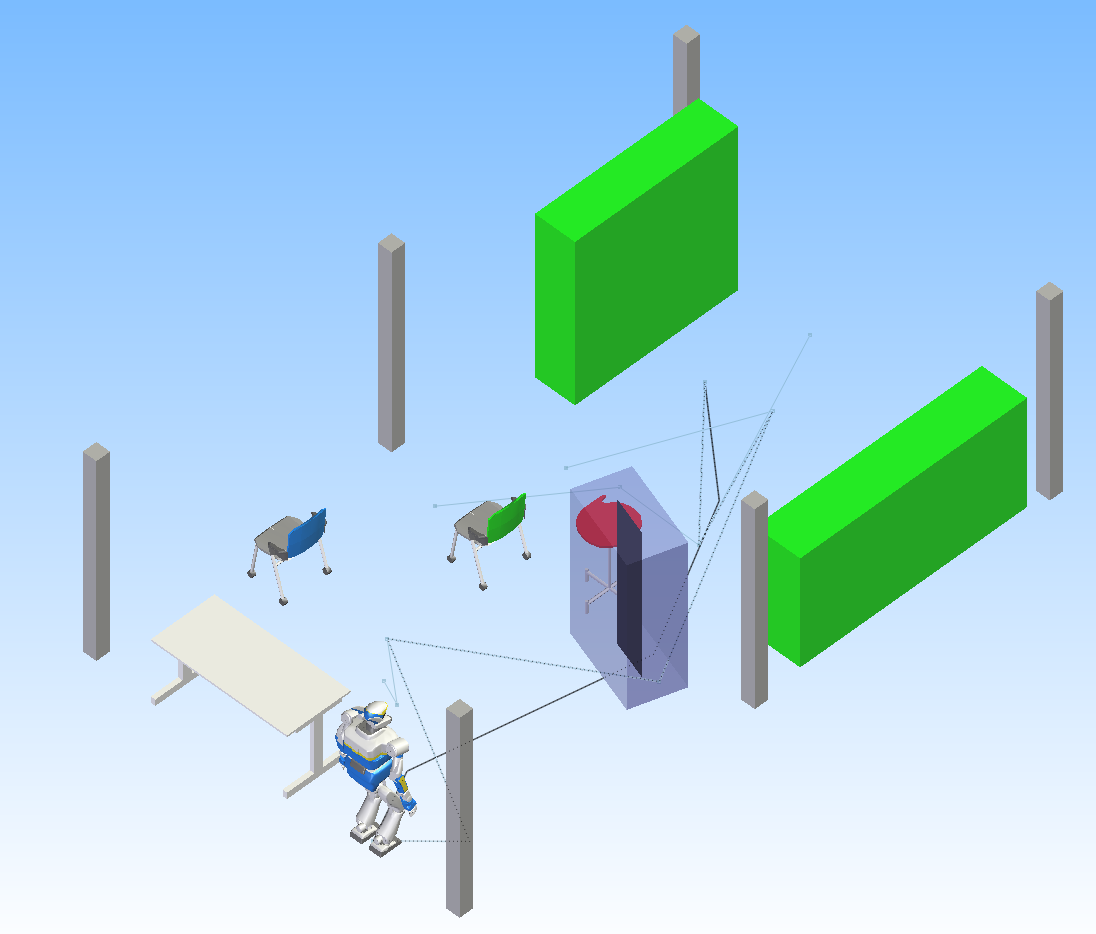
\includegraphics[width=.8\linewidth]{src/chap1-roboptim/optim-length.png}
  \end{center} \caption{Exemples d'optimisation d'une trajectoire en
  présence d'obstacles. \label{fig:obstacle}}
\end{figure}

\begin{figure}[htbp]
  \begin{center}
    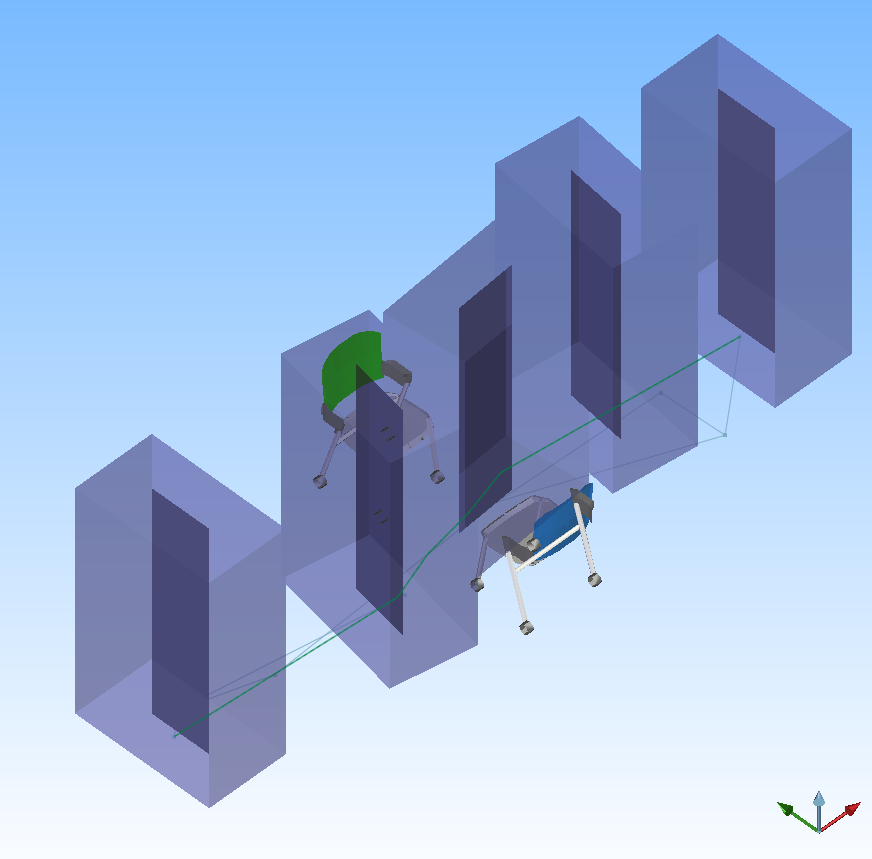
\includegraphics[width=.45\linewidth]{src/chap1-roboptim/two-chairs.png}
    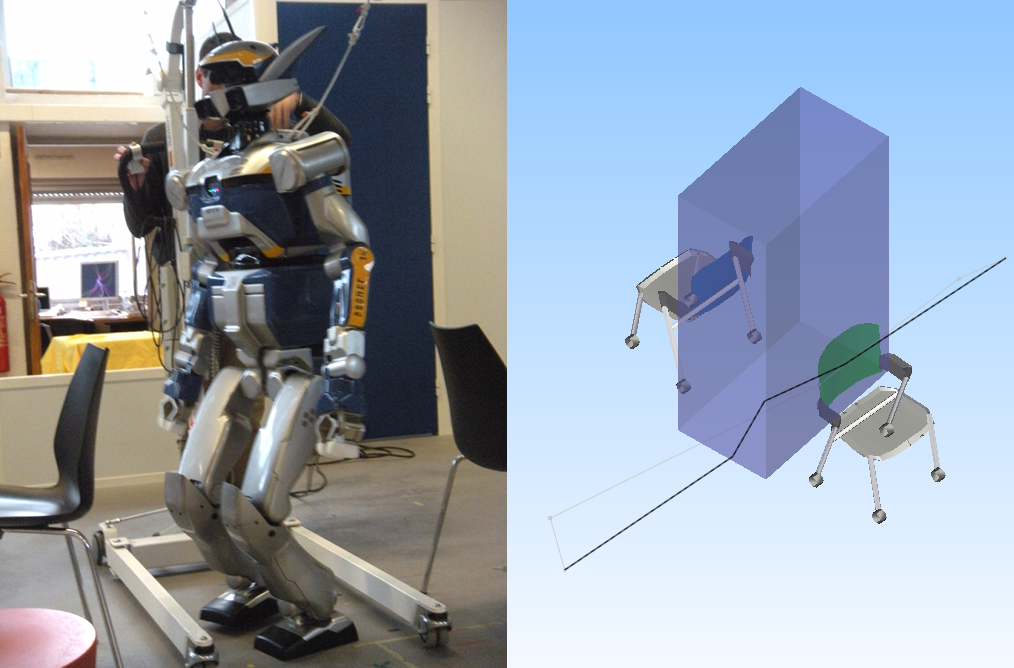
\includegraphics[width=.45\linewidth]{src/chap1-roboptim/hrp2-two-chairs.png}
  \end{center}
 \caption{Résultat expérimental sur le robot humanoïde
   HRP-2. \label{fig:results}}
\end{figure}

\begin{table}
  \begin{center}
    \begin{tabular}{|c|l l l|l|}
      \hline \bf Scenarii & Planification & Optimisation &
      \emph{Calcul complet}\\ \hline \bf Passage entre deux chaises &
      8.58s & 47.22s & \emph{2 min 05.55 s}\\ \hline \bf Salle
      réaliste avec de nombreux obstacles & 4.14 s & 1 min 9.35 s &
      \emph{4 min 5.11 s}\\ \hline
    \end{tabular}
  \end{center}
  \caption{Temps de calculs. Le temps de calcul complet comprends la
    planification, l'optimisation et la phase de génération de
    mouvement corps complet.\label{tab:benchmarks}}
\end{table}


\section{Conclusion}
\label{sec:chap1_conclusion}

Ce chapitre a été dédié à la conception d'une modélisation orientée
objet pour la résolution de problèmes d'optimisation numériques ainsi
qu'à son implémentation, la suite logicielle RobOptim. Après avoir
observé les solveurs disponibles sur le marché, on peut facilement
s'apercevoir de l'écart considérable entre d'un côté la théorie
mathématique et son implémentation en pratique. En pratique, chaque
solveur vient avec son formalisme, ses interfaces et force ses
utilisateurs à apprendre une nouvelle formalisation pour chaque
nouveau solveur utilisé. De ce fait, réaliser des comparaisons est
malaisé, l'apprentissage inutilement difficile et les interfaces
souvent peu claires ou mal documentées. En fournissant un point
d'entrée pour plusieurs algorithmes, il n'y a qu'une interface et un
paradigme à expliquer ce qui présente un gain net vis-à-vis de
l'approche habituelle. De plus, de nombreux outils sont utiles en
optimisation tout en étant décorrélés de l'algorithme de
résolution. Le calcul des gradients par différences finies est un bon
exemple. Dans RobOptim, il a été intégré à la fois pour pouvoir éviter
d'avoir à calculer les gradients de manière analytique, mais il peut
également servir à vérifier le gradient analytique. Du point de vue du
logiciel, l'accent a été mis sur la création d'un ensemble de
bibliothèques logicielles simples à utiliser et assurant la correction
du problème posé. Cette correction passe par l'utilisation d'un
système de typage fort permettant de détecter à la compilation les
problèmes qui peuvent se poser. En effet, RobOptim interdit, à la
compilation, la construction d'un problème invalide: si certains
gradients sont manquants ou bien si certains types de fonction sont
incorrects, la compilation du fichier échouera, car les contraintes de
typage ne seront pas respectées. Malgré ce système de typage imposant
des règles strictes, une grande flexibilité a été gardée dans le choix
de l'algorithme qui peut s'effectuer à l'exécution. Le système de
plug-in de RobOptim permettant de charger les algorithmes
dynamiquement pendant l'exécution du programme. La suite logicielle a
été validée sur un exemple réel de robotique qu'est l'optimisation de
trajectoire de marche pour un robot humanoïde.
